\section{Bayesian statistics and Markov chain Monte Carlo}

In the following section we will briefly discuss the main features of a Bayesian statistical approach, comparing it with the classical inferential statistics. Then, we will present a class of techniques used to practically perform Bayesian inference, the Markov chain Monte Carlo (commonly denoted with the acronym MCMC), discussing some of the possible implementations and properties of these methods.
\subsection{Bayes' formula}
The basis of Bayesian statistics can be found in the simple Bayes' formula. Let us consider an event space $\Omega$, a sigma-algebra $\mathcal{A}$, a probability measure $P$ and the probability space $(\Omega, \mathcal{A}, P)$. If $A$ and $B$ are two events in $\Omega$, the probability of the intersection of $A$ and $B$ is given by
\begin{equation}
\begin{aligned}
	P(A, B) &= P(A|B)P(B) \\
	&= P(B|A)P(A).
\end{aligned}
\end{equation}
The equivalence between the two formulations leads to Bayes' formula
\begin{equation}\label{eq:BayesRule}
	P(A|B) = \frac{P(B|A)P(A)}{P(B)}.
\end{equation}
In Bayes' formula, $P(A|B)$ is a probability distribution, therefore its integral has to be equal to one. Therefore, one can rewrite Bayes' rule disregarding the value of $P(B)$ as
\begin{equation}
	P(A|B) \propto P(A)P(B|A).
\end{equation}
The exact value of the probability distribution can be therefore obtained by normalization as
\begin{equation}
	P(A|B) = \frac{P(A)P(B|A)}{\int_{\Omega}P(A)P(B|A)}.
\end{equation}
The quantities appearing in \eqref{eq:BayesRule} are commonly referred to as
\begin{itemize}
	\item posterior distribution $P(A|B)$,
	\item prior distribution $P(A)$,
	\item likelihood $P(B|A)$.
\end{itemize} 
The probability distribution of $A$ is often the object of Bayesian inference and the event $B$ is an observable quantity related to $A$. Then the likelihood $P(B|A)$ is not a probability distribution but the likelihood the observations of $B$ have with respect to $A$. Therefore, in order to avoid misinterpretations, we will denote in the following the likelihood by $\diffL(B|A)$. Moreover, we will adopt in the following sections the notation $\prior$ for the prior and $\pi$ for the posterior distributions, thus obtaining
\begin{equation}
	\pi(A|B) \propto \prior(A) \diffL(B|A).
\end{equation}

\subsection{Parametrized models}
Bayes' formula opens a new perspective to statistical modeling with respect to the classical inferential standards. In particular, parametrized models are particularly suited to a Bayesian approach. Let us consider a parametrized model for predicting the outcome of an experiment. Let us denote by $\theta$ the parameter driving the experiment and by $X$ a random variable representing its outcome. Let us consider for simplicity $\theta$ as a vector of $\R^{N_p}$, where $N_p$ is the dimension of the parameter space. We will then denote by $\theta_i$ the $i$-th component of the parameter, with $i = 1, \ldots, N_p$. For instance, we could consider the toss of a coin and estimate its probability to fall on one of the two side as $\theta$, or more complicated physical models influenced by an intractable source of noise.

In the classical statistic approach we would state an hypothetical distribution for $X$ depending on the parameter (e.g., $X \sim \mathcal{N}(\theta_1, \theta_2)$). Then, let us suppose that a set of observation $\mathcal{Y}_i = \{y_0, y_1, \ldots, y_i\}$, $i = 1, \ldots, N_d$, of the outcome of the experiment is available. We can consider these observations to be produced by a random variable $Y$ representing a quantity connected to the random variable $X$ by a law, that we denote by $f$, and biased by a measurement error, that we denote by $\epl$. For instance, we could consider the following additive observational model 
\begin{equation}\label{eq:GaussianNoise}
	Y \sim f(X) + \epl, \quad \epl \sim \mathcal{N}(0, \Gamma).
\end{equation}
Given this background, there are many techniques available in the classical approach to compute an estimator $\hat \theta$ of the true parameter and to state a measure of the uncertainty the statistical model has on the estimator. In particular, one can compute analytically quantities such as the mean square error (MSE) of the estimator or give confidence intervals on $\theta$ such that its true value falls in the interval up to a threshold probability.

In the Bayesian frame the estimation of $\theta$ follows a completely different philosophy. The outcome of the Bayesian inference is neither a value of the parameter nor a set of values in which it is likely to be  included, but it is a \textit{probability distribution}. Maintaining the notation introduced above, Bayes' formula in this frame reads
\begin{equation}
	\pi(\theta|\mathcal{Y}_i) \propto \prior(\theta) \diffL(\mathcal{Y}_i|\theta).
\end{equation}
Let us analyze separately the two terms of this equation.
\begin{itemize}
	\item Given a set of observations $y_i$, $i = 1, \ldots, N_d$, and an observational model the likelihood $\diffL(Y|\theta)$ can be evaluated. For example, in the Gaussian case introduced in \eqref{eq:GaussianNoise} analytical formulas for the likelihood are available.
	\item The prior distribution $\prior(\theta)$ has to be established before the observation are obtained. This is a crucial part of the process of Bayesian inference, since in practice if the prior distribution is wrong or inadmissible, the obtained posterior may be negatively affected by this choice.
\end{itemize}
The two approaches give both equally valid results but in a completely different spirit. While in classical statistics the model driving an experiment is predetermined and its parameters are computed using observations, in the Bayesian frame the object of study is the model behind the parameter itself, which is revealed by the observations.

\subsubsection{An example: parametrized differential equations}\label{sect:exBayes}

In this paragraph we present a simple example that is useful to understand Bayesian inference of parameters in general and the scope of this work in particular. Let us consider the probability space $(\Omega, \mathcal{F}, P)$, a one-dimensional standard Wiener process $\left\{W(t)\right\}_{t\geq 0}$ and a filtration $\left\{\mathcal{F}(t)\right\}_{t\geq 0}$ such that $W(t)$ is $\mathcal{F}(t)$ measurable. Moreover, let us consider the following one-dimensional stochastic differential equation (SDE)
\begin{equation}\label{eq:exSDE}
\begin{aligned}
	dX(t) &= \lambda X(t) \dd t + \mu X(t) dW(t), && 0 < t < T, \\
	X(0) &= X_0, && X_0 \in \R,
\end{aligned}
\end{equation}
where $\lambda, \mu$ are real parameters and $X_0$ is a random variable. It is known that under the hypotheses of It\^o calculus the solution of \eqref{eq:exSDE} is given by
\begin{equation}
	X(t) = X_0 \exp\left(\left(\lambda - \frac{1}{2}\mu^2\right)t + \mu W(t)\right),
\end{equation}
which is a stochastic process often referred to as \textit{geometric Brownian motion}. This equation and its solution have extensively been studied  in numerous applications. For example, it used as a simple financial tool in order to model option or stock pricing, with the parameter $\lambda$ which is often referred to as the \textit{drift} and the diffusion coefficient $\mu$ as the \textit{volatility}. Given the model described by \eqref{eq:exSDE}, we may be interested in inferring the value of one, or more, of its parameters. 

Let us consider the following assumptions
\begin{itemize}
	\item $X_0$ is a known real value, 
	\item the drift coefficient $\lambda$ is known a priori,
	\item the diffusion coefficient $\mu$ is unknown but a prior distribution $\prior(\mu)$ has been stated,
	\item the value of the solution $X(t)$ is observable at a set of times $t_i$, $i = 1, \ldots, N_d$, such that $t_{N_d} = T$, with a zero-mean additive Gaussian measurement noise $\epl$, i.e., the observations $y_i$, are given by
	\begin{equation}
		y_i = x(t_i) + \epl_i, \quad \epl_i \iid \mathcal{N}(0, \sigma^2), \quad  \sigma \in \R, \quad i = 1, \ldots, N_d,
	\end{equation}  
	where we denote by $x(t_i)$ a realization of $X$ evaluated at time $t_i$.
\end{itemize}
Let us denote as $\mathcal{Y}_i$ the set of all the observations $y_i$ up to time $t_i$. We are interested in estimating the value of the parameter $\mu$. In a Bayesian frame, this corresponds to providing a distribution $\pi$ conditional to the observation following Bayes' rule, i.e.,
\begin{equation}
	\pi(\mu|\mathcal{Y}_i) \propto \prior(\mu) \diffL(\mathcal{Y}_i|\mu).
\end{equation}
In this simple frame, the knowledge of the analytical form of the solution and of the measurement error gives us an exact notion of the model connecting the parameter and the observations. Hence, for each choice of the value of $\mu$ it is possible to evaluate the likelihood function $\diffL$ as follows
\begin{equation}
	\diffL(\mathcal{Y}_{N_d}|\mu) = (2\pi\sigma^2)^{-N_d/2}\prod_{k = 1}^{N_d}\E\left[\exp(-\frac{\sigma^2}{2}(X(t_k) - y_k)^2)\right],
\end{equation}
where we omitted the implicit dependence of the process $X$ on $\mu$. Furthermore, if the prior distribution $\prior$ admits a density in closed form, it is possible to evaluate it on any choice of $\mu$. Therefore, it is possible to compute for each value of $\mu$ the value of the posterior distribution associated with the available set of measurements. 

In this simple example the analytical form of any of the quantities of Bayes' formula and the small dimension of the parameter space imply that with a low effort it is possible to determine the value of the posterior distribution. In general this is not true, and as we will show in the next sections fine Monte Carlo techniques have been proposed to generate samples from any distribution. 

\subsection{Markov chain Monte Carlo methods}

Markov chain Monte Carlo methods (MCMC) are a class of techniques used to perform Bayesian analyses \cite{Gil05, KaS05}. In the following we will present the main idea behind the method as well as some examples of their implementation. 

Let us consider a model which has a random variable $X$ as its outcome parametrized by a parameter $\theta$ and a set of observations $\mathcal{Y}_i = \left\{y_1, y_2, \ldots, y_i\right\}$, $i = 1, \ldots, N_d$, providing information regarding $X$. Then, thanks to Bayes' rule, we can construct the posterior distribution of $\theta$ by Bayes' rule
\begin{equation}
	\pi(\theta|\mathcal{Y}_i) \propto \prior(\theta) \diffL(\mathcal{Y}_i|\theta).
\end{equation}
As in the previous paragraphs, let us assume that $\theta$ is a real-valued parameter of dimension $N_p$. If the parameter space has a high dimension, it is computationally expensive exploring all the possible values in order to build the posterior distribution, especially if evaluating the model connecting $\theta$ and the random variable $X$ is non-trivial. If we are interested in knowing the expectation of some measurable function $g\colon \R^{N_p} \to \R$ of $\theta$ we can proceed by the following Monte Carlo evaluation
\begin{equation}\label{eq:MonteCarloMCMC}
	 \E\left[g(\theta)\right]= \int_{\R^{N_p}} g(\theta)\pi(\dd\theta|\mathcal{Y}_i) \approx \frac{1}{N}\sum_{k = 1}^{N} g(\theta^{(k)}),
\end{equation}
where $\theta^{(k)}$, $k = 1, \ldots, N$, is a set of realizations of $\theta$. While the equality in the equation follows from the definition of expectation, there is no guarantee that the Monte Carlo estimator will be a good approximation of the expectation regardless of the samples. MCMC techniques consist in generating samples such that the Monte Carlo approximation is valid without exploring the whole parameter space,  which would lead to an unaffordable computational time on any modern computer. As the name of the methods suggests, given an initial guess $\theta^{(0)}$, MCMC builds a discrete Markov chain $\{\theta^{(i)}\}_{i\geq 0}$ such that the Monte Carlo approximation in \eqref{eq:MonteCarloMCMC} is valid. Formally, this is achieved considering a \textit{transition kernel} $P$ which given the current element of the chain $\theta^{(i)}$ produces the next guess $\theta^{(i+1)}$. Under a set of assumptions on $P$ \cite{KaS05}, we have the theoretical guarantee that the samples $\theta^{(i)}$ are drawn from the same \textit{stationary distribution} for $i$ large enough. We can build many transition kernels having this property, and any valid choice of $P$ leads to a different MCMC method. In the following, we will present the widely-used \textit{Metropolis-Hastings} algorithm, as well as two of its variants that were necessary for our work.

\subsubsection{Metropolis-Hastings algorithm}
\begin{algorithm}[t]
	\caption{Metropolis-Hastings.}
	\label{alg:MH}
	\KwData{$\theta^{(0)} \in \R^{N_p}, N \in \N_0$.}
	Compute $\pi(\theta_0)$ \;
	\For{$i = 0, \ldots, N$}{
		Draw $\vartheta$ from $q(\theta^{(i)}, \cdot)$ \;
		Compute the acceptance probability $\alpha(\theta^{(i)}, \vartheta)$ as in \eqref{eq:MHalpha} \;
		Draw $u$ from $\mathcal{U}(0, 1)$ \;
		\eIf{$\alpha > u$} {
			Accept $\vartheta$, set $\theta_{i+1} = \vartheta$ \; 
		} {
		Set $\theta^{(i+1)} = \theta^{(i)}$\;
	}
}
\end{algorithm}
In this paragraph we will introduce one of the most successful MCMC methods, the Metropolis-Hastings method (MH). In MH, the samples forming the Markov chain are generated following a \textit{proposal distribution} $q\colon \R^{N_p} \cross \R^{N_p} \to \R^+$ which satisfies the condition
\begin{equation}
	\int_{\R^{N_p}}q(x, y)\dd y = 1,
\end{equation}
thus $q$ is a probability distribution in its second argument. Given the current guess $\theta^{(i)}$, MH proposes the new element of the Markov Chain drawing a value $\vartheta$ from $q(\theta^{(i)}, \cdot)$. The new guess is not automatically accepted as the new element $\theta^{(i+1)}$ of the Markov chain, but it is accepted with a probability, that we denote by $\alpha(\theta^{(i)}, \theta^{(i+1)})$. Formally, the transition kernel $P_{\MH}$ representing the move made by MH from $\theta^{(i)}$ to $\theta^{(i+1)}$ is given by \cite{MLR16}
\begin{equation}
	P_{\MH}(\theta^{(i)}, \theta^{(i+1)}) = \alpha(\theta^{(i)}, \theta^{(i+1)})q(\theta^{(i)},\theta^{(i+1)}) + \delta_{\theta^{(i)}}(\theta^{(i+1)})\rho(\theta^{(i)}),
\end{equation}
where $\delta_x$ is the Dirac delta centered in $x$ and $\rho$ is defined as
\begin{equation}
	\rho(\theta^{(i)}) \defeq 1 - \int_{\R^{N_p}}\alpha(\theta^{(i)}, x)q(\theta^{(i)}, x)\dd x.
\end{equation}
In words, the expression of the transition kernel $P_{\MH}$ is equivalent to stating that the new guess $\vartheta$ generated from the proposal distribution is accepted with probability $\alpha$ and rejected with probability $1 - \alpha$. Imposing that $P_{\MH}$ satisfies the hypotheses that guarantee the convergence of MCMC, we can get the expression of the acceptance probability in closed form as 
\begin{equation}\label{eq:MHalpha}
	\alpha(\theta^{(i)}, \vartheta) = \min\left\{\frac{\pi(\vartheta)q(\vartheta, \theta^{(i)})}{\pi(\theta^{(i)})q(\theta^{(i)}, \vartheta)}, 1\right\}.
\end{equation}
As it is possible to remark from its pseudo-code, given in Algorithm \ref{alg:MH}, MH is extremely simple to implement on a computer in any programming language. In fact, the only choice left to the user of a MH algorithm is the proposal distribution $q(x,y)$. Unfortunately, this choice could impact negatively the behavior of MH, slowing dramatically its convergence towards the stationary distribution of the Markov chain. Let us first remark that if the proposal distribution is a symmetric function in its two arguments, i.e., $q(x, y) = q(y, x)$,  the expression of the acceptance probability simplifies to
\begin{equation}\label{eq:MHalphasym}
	\alpha(\theta^{(i)}, \vartheta) = \min\left\{\frac{\pi(\vartheta)}{\pi(\theta^{(i)})}, 1\right\}.
\end{equation}
For example, a Gaussian proposal distribution centered in $\theta^{(i)}$ with covariance matrix $\Sigma$ in $\R^{N_p\times N_p}$ is a common choice for $q(x, y)$. In this case, the proposal distribution is given up to a normalization constant by
\begin{equation}\label{eq:gaussianProp}
	q(x, y) \propto \exp(-\frac{1}{2}(x - y)^T\Sigma^{-1}(x - y)).
\end{equation}
In this work, we mainly used a Gaussian proposal distribution, therefore the acceptance probability will be of the form \eqref{eq:MHalphasym}. 

Two main issues have to be taken into account before moving on to the practical applications of MH we considered for this work.
\begin{enumerate}
	\item What is a good choice for the proposal function $q(x, \cdot)$?
	\item How can we modify MH in case it is not possible, or not practical, to evaluate the posterior distribution $\pi(\theta)$?
\end{enumerate}
In the following paragraphs we will present two approaches to modify MH targeting these two questions. 

\subsubsection{An adaptive approach}
\begin{algorithm}[t]
	\caption{Robust adaptive Metropolis.}
	\label{alg:RAM}
	\KwData{$\theta^{(0)} \in \R^{N_p}, \: N \in \N_0, \: S_0 \in \R^{N_p \times N_p}, \: \alpha^* \in (0, 1)$.}
	Compute $\pi(\theta_0)$ \;
	\For{$i = 0, \ldots, N$}{
		Draw $z$ from $Z \sim \mathcal{N}(0, I)$ \;
		$\vartheta = \theta^{(i)} + S_i z$ \; 
		Compute the acceptance probability $\alpha(\theta^{(i)}, \vartheta)$ as in \eqref{eq:MHalpha} \;
		Draw $u$ from $\mathcal{U}(0, 1)$ \;
		\eIf{$\alpha > u$} {
			Accept $\vartheta$, set $\theta_{i+1} = \vartheta$ \; 
		} {
		Set $\theta^{(i+1)} = \theta^{(i)}$\;
		}
		Compute $S_{i+1}$ as in \eqref{eq:RAMupdate} \;
	}
\end{algorithm}
In the frame of MH algorithms, it is important to have a control on the \textit{acceptance ratio}, i.e., the ratio of new proposed values $\vartheta$ that are included in the Markov chain $\{\theta^{(i)}\}_{i\geq 0}$. In the MH frame, the acceptance ratio depends on the chosen proposal distribution, as if the new guess produced via the proposal distribution have a low probability of being accepted, a low value of acceptance ratio will result from the algorithm. If the initial proposal distribution does not provide with acceptable values $\vartheta$, it may be necessary to tune it during the advancement of MH. An algorithm which targets this issue is the robust adaptive Metropolis (RAM) \cite{Vih12}. 

Let us consider the case a Gaussian proposal distribution $q(x,y)$ as in \eqref{eq:gaussianProp}. At the $n$-th step of MH the new guess $\vartheta$ of the parameter is given by
\begin{equation}
\vartheta = \theta^{(n)} + z, \quad Z \sim \mathcal{N}(0, \Sigma),
\end{equation}
where $\Sigma$ is the covariance matrix. It is possible to build a sequence of matrices such that the convergence properties of MH are not spoiled and the acceptance rate is asymptotically equal to a given value $\alpha^*$ \cite{Vih12}. This is obtained through the following update 
\begin{equation}
\vartheta = \theta_k + S_n z_n, \quad Z_n \sim \mathcal{N}(0, I),
\end{equation}
with $S_n$ a lower triangular positive definite matrix and $I$ the identity matrix. Given an initial choice $S_0$, the matrix $S_n$ is updated at each iteration with a lower triangular matrix $S_{n+1}$ satisfying
\begin{equation}\label{eq:RAMupdate}
S_{n+1}S_{n+1}^T = S_n\left(I + \eta_n\left(\alpha(\theta^{(n)}, \vartheta) - \alpha^*\right)\frac{z_nz_n^T}{z_n^Tz_n}\right)S_n^T.
\end{equation}
Hence, we can compute $S_{n+1}$ as the Cholesky factorization of the right hand side. Let us remark that this update has to be performed at each iteration of RAM, both in case $\vartheta$ is accepted and rejected. The sequence $\left\{\eta_n\right\}_{n\geq 1}$ can be any sequence decaying to zero with $n$. In this work, we consider \cite{Vih12}
\begin{equation}
\eta_n = n^{-\gamma}, \quad 0.5 < \gamma \leq 1.
\end{equation}
Often the computational cost needed for the evaluation of the posterior distribution is high with respect to the dimension $N_p$ of the parameter space. Therefore, performing a Cholesky factorization at each iteration, which has a complexity of $\OO(N_p^3)$, does not spoil the performances of RAM with respect to a standard MH. In Algorithm \ref{alg:RAM} we give the pseudo-code for the RAM update.

We now present a numerical example showing the optimal behavior of RAM. Let us consider a two-dimensional real random variable $X$ whose distribution admits the following density
\begin{equation}\label{eq:RAMtestPi}
	\pi(X) \propto \exp(-10(X_1^2 - X_2)^2 - (X_1 - 0.25)^4),
\end{equation}
where we denoted by $X_i$, $i = 1, 2$ the two components of $X$ and we omitted the normalization constant. This distribution is widely used to test MCMC algorithms \cite{KaS05}. We then consider a real value $\sigma$ in the set $\{0.01, 0.5, 2.0\}$ and target the distribution defined by \eqref{eq:RAMtestPi} either using a standard MH with the proposal distribution given by a zero-centered normal distribution with covariance $\Sigma = \sigma^2 I$, or using RAM with the same choice of covariance structure as an initial guess and $\alpha^* = 0.4$. We run $N = 5000$ iterations of both algorithms and register all the guesses they produce as well as the final acceptance ratio. Results (Figure \ref{fig:RAMexample}) show that for the $\sigma = 0.01$ and $\sigma = 2.0$ standard MH fails to properly describe the posterior distribution, either accepting too many guesses and partially describing the posterior, or refusing almost all guesses therefore obtaining an insufficient number of samples. On the other hand, RAM adapts the step and for any choice of $\sigma$ the samples we obtain are equally good, with an acceptance ratio near to $\alpha^*$ (Table \ref{tab:RAMalphaStar}).

\begin{table}[H]
	\centering
	\begin{tabular}{cccc}
		\toprule
		MCMC & $\sigma = 0.01$ & $\sigma = 0.5$ & $\sigma = 2.0$ \\ 
		\midrule
		MH & 0.96  & 0.35  & 0.06  \\
		RAM & 0.43 & 0.40 & 0.38 \\
		\bottomrule
	\end{tabular}
	\caption{Acceptance ratios for MH and RAM with posterior distribution \eqref{eq:RAMtestPi}}.
	\label{tab:RAMalphaStar}
\end{table}

\begin{figure}[t]
	\centering
	\begin{subfigure}{0.32\linewidth}
		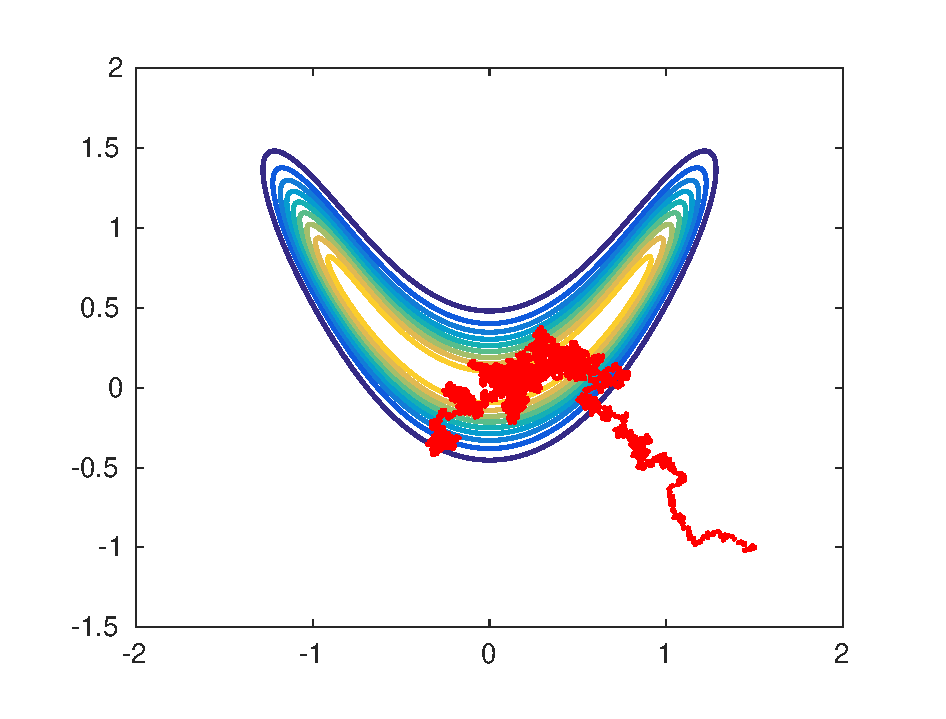
\includegraphics[width=1\linewidth]{plots/MHvsRAM/MH_small}
	\end{subfigure}
	\begin{subfigure}{0.32\linewidth}
		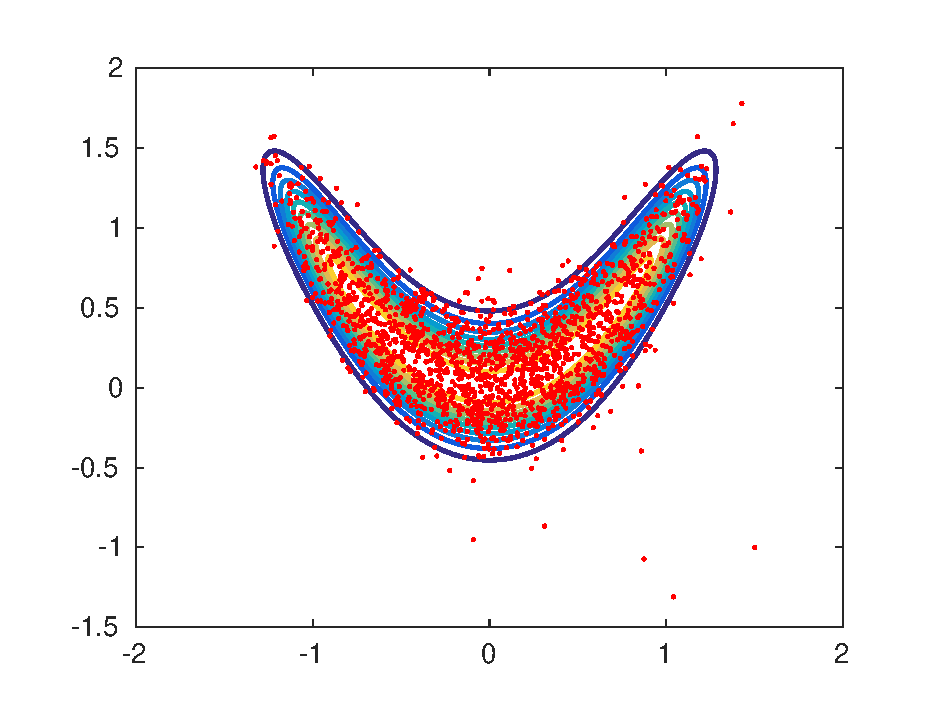
\includegraphics[width=1\linewidth]{plots/MHvsRAM/MH_medium}
	\end{subfigure}
	\begin{subfigure}{0.32\linewidth}
		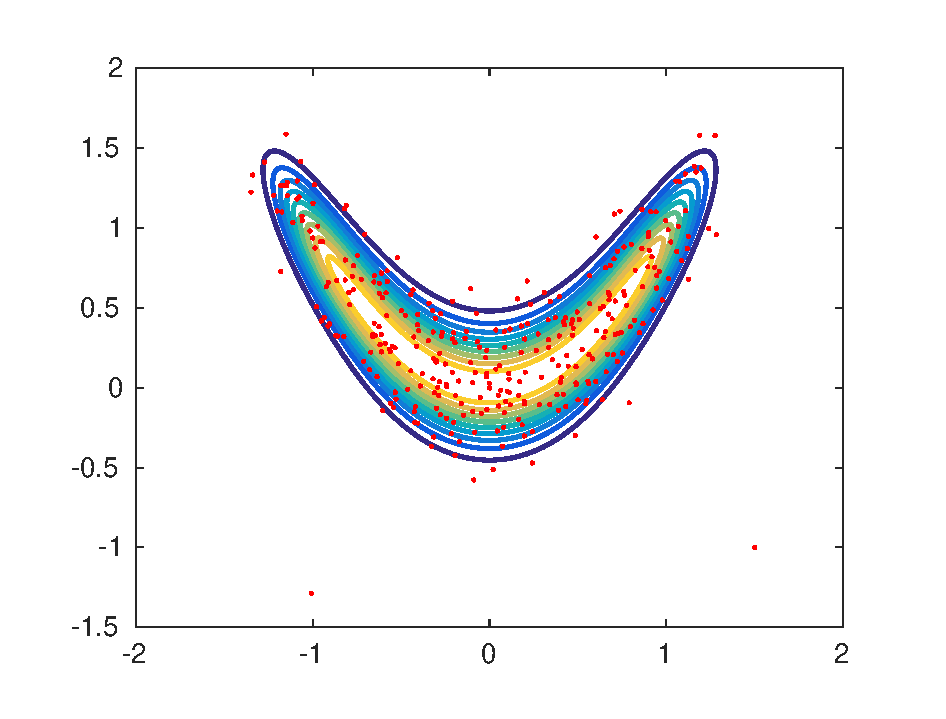
\includegraphics[width=1\linewidth]{plots/MHvsRAM/MH_big}
	\end{subfigure}
	
	\begin{subfigure}{0.32\linewidth}
		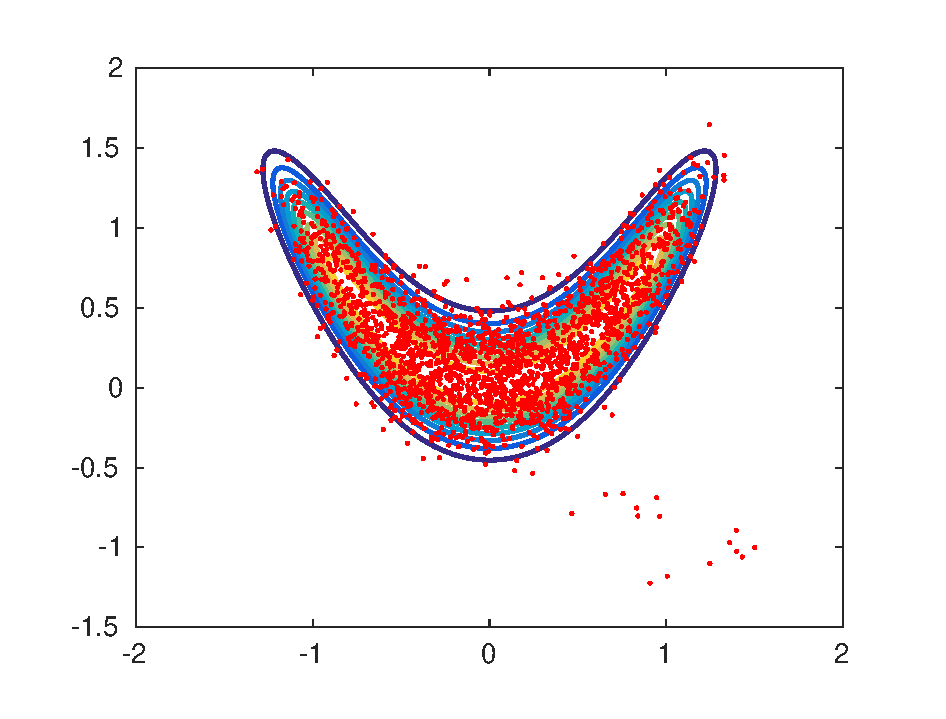
\includegraphics[width=1\linewidth]{plots/MHvsRAM/RAM_small}
	\end{subfigure}
	\begin{subfigure}{0.32\linewidth}
		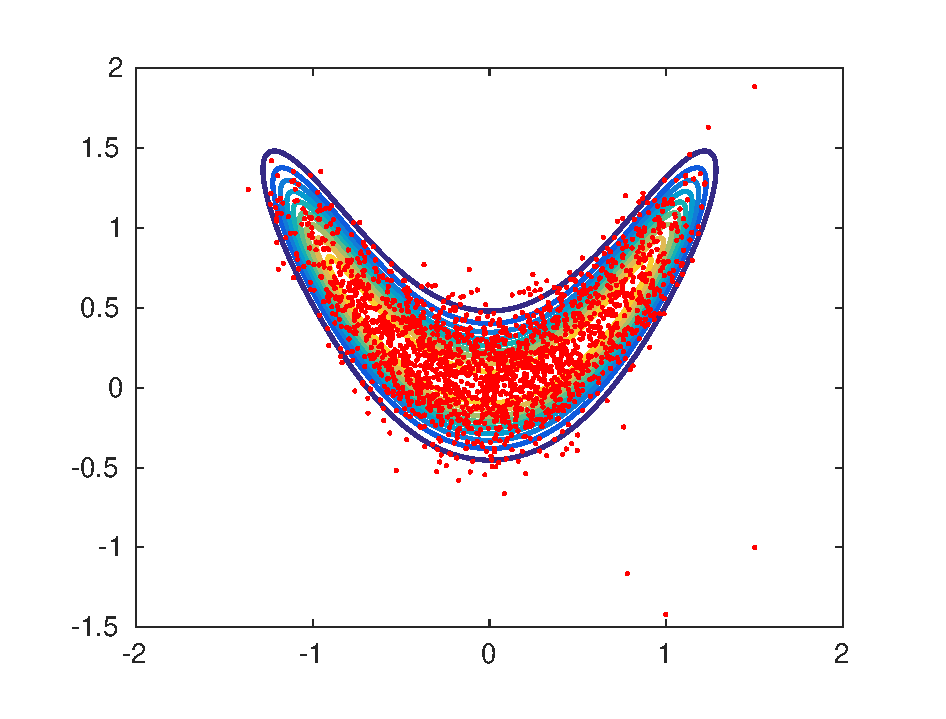
\includegraphics[width=1\linewidth]{plots/MHvsRAM/RAM_medium}
	\end{subfigure}
	\begin{subfigure}{0.32\linewidth}
		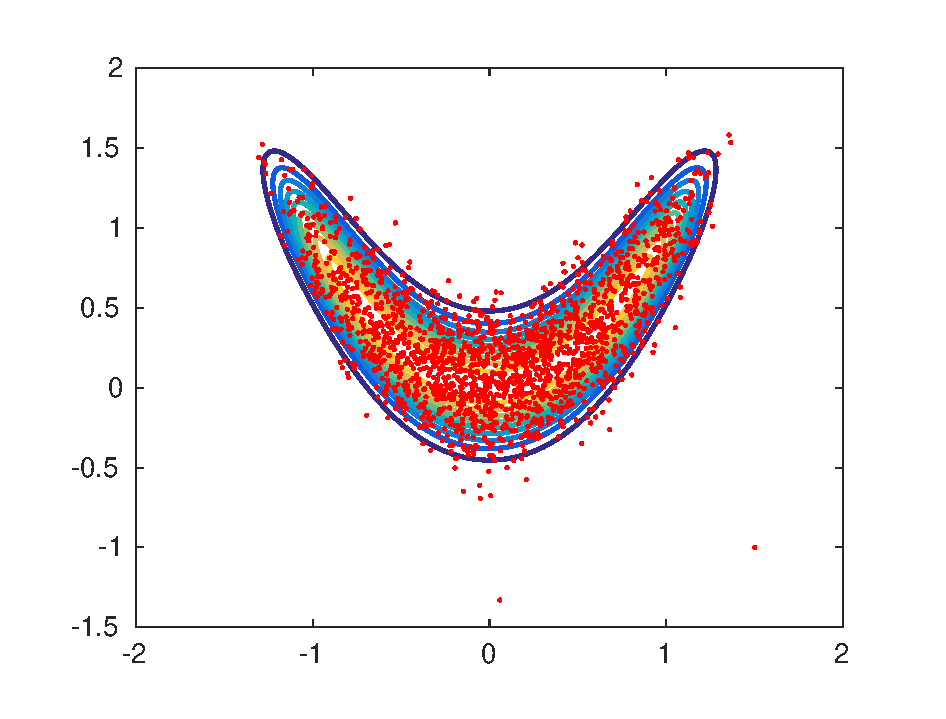
\includegraphics[width=1\linewidth]{plots/MHvsRAM/RAM_big}
	\end{subfigure}
	\caption{Samples produced by MH and RAM for the distribution \eqref{eq:RAMtestPi}. The contour lines of the density function are plotted for all the sets of results. In the first row we show the results obtained with MH for a normal update with covariance $\Sigma = \sigma^2 I $ with $\sigma = \{0.01, 0.5, 2.0\}$ from left to right. In the second row we show the results obtained with RAM with the same values of $\Sigma$ as an initial guess of the covariance structure. }
	\label{fig:RAMexample}
\end{figure}

\subsubsection{Pseudo-marginal Metropolis-Hastings} \label{sec:MCWM}
\begin{algorithm}[t]
	\caption{Monte Carlo within Metropolis.}
	\label{alg:MCWM}
	\KwData{$\theta^{(0)} \in \R^{N_p}, \: N \in \N_0$.}
	Compute $\pi(\theta_0)$ \;
	\For{$i = 0, \ldots, N$}{
		Draw $\vartheta$ from $q(\theta^{(i)}, \cdot)$ \;
		Compute the estimators $\pi_M(\theta^{(i)}, \xi)$ and $\pi_M(\vartheta, \xi)$ as in \eqref{eq:MCWMestimators} \;
		Compute the acceptance probability $\alpha_M(\theta^{(i)}, \vartheta)$ as in \eqref{eq:MCWMalpha}\;
		Draw $u$ from $\mathcal{U}(0, 1)$ \;
		\eIf{$\alpha > u$} {
			Accept $\vartheta$, set $\theta_{i+1} = \vartheta$ \; 
		} {
		Set $\theta^{(i+1)} = \theta^{(i)}$\;
	}
}
\end{algorithm}
In this paragraph we discuss the second issue presented above. Let us consider the case in which it is not possible to evaluate the posterior distribution $\pi(\theta)$, or it is too computational expensive. For instance, in the example we provided in Section \ref{sect:exBayes} the analytical solution of the SDE is computable. If we have a general equation which does not admit a closed-form solution, it is not possible to evaluate the likelihood function. Therefore, the standard MH algorithm and its adaptive version RAM are not applicable.

An algorithm that has been proposed to overcome this issue is the so-called \textit{pseudo-marginal} MCMC \cite{DPD15}, which is also known as particle Markov chain Monte Carlo (PMCMC) \cite{ADH10}. The main idea of the proposed pseudo-marginal algorithms is modifying the target of the algorithm to a distribution $\pi(\theta, \xi)$ that admits $\pi(\theta)$ as a marginal distribution and that is easier than $\pi(\theta)$ to evaluate. Then, we can compute an unbiased Monte Carlo approximation $\pi_M(\theta)$ of the marginal distribution as
\begin{equation}\label{eq:MCWMestimators}
	\pi_M(\theta) = \frac{1}{M} \sum_{i = 1}^{M} \pi(\theta, \xi^{(i)}),
\end{equation}
where the values $\xi^{(i)}$ are realizations of the random variable $\xi$. The acceptance probability $\alpha_M$ has then the same form of $\alpha$ in the standard MH, with $\pi_M(\theta)$ instead of the true marginal distribution, i.e.,
\begin{equation}\label{eq:MCWMalpha}
	\alpha_M(\theta^{(i)}, \vartheta) = \min\left\{\frac{\pi_M(\vartheta)q(\vartheta, \theta^{(i)})}{\pi_M(\theta^{(i)})q(\theta^{(i)}, \vartheta)}, 1\right\}.
\end{equation}
The pseudo-code of the resulting algorithm is shown in Algorithm \ref{alg:MCWM}. Let us remark that if the estimator $\pi_M(\theta^{(i)})$ at the $i$-th iteration of MCMC is computed at each iteration and not recycled from the previous iterations, the resulting algorithm is often referred to as Monte Carlo within Metropolis (MCWM) \cite{AnR09} or noisy pseudo-marginal Metropolis \cite{MLR16}. Even though recomputing the estimator may be computationally expensive, the resulting Markov chain has an higher acceptance ratio, i.e., it explores the relevant values of the parameter $\theta$ faster, therefore defining better the posterior distribution. The main issue that has been addressed by the research on this kind of pseudo-marginal algorithms is whether the invariant distribution of the Markov chain converges to the marginal posterior distribution of the random variable $\theta$. It has been shown \cite{AnR09, MLR16} that under appropriate assumptions the following properties are valid
\begin{enumerate}
	\item the transition kernel $P_M$ given by \eqref{eq:MCWMalpha} converges to an invariant distribution $\pi_M$ with the number of iterations $N$ of MCMC if the number of Monte Carlo draws $M$ is large enough \cite[Theorem 9]{AnR09},
	\item the invariant distribution $\pi_M$ obtained with MCWM converges to the true marginal distribution $\pi$ if $M$ tends to infinity \cite[Theorem 4.1]{MLR16},
	\item under stronger assumptions, it is possible to obtain convergence rates of $\pi_M$ to $\pi$ with respect to $M$ \cite[Theorem 4.2 and Proposition 4.1]{MLR16}.
\end{enumerate}
Let us consider the example provided in Section \ref{sect:exBayes}. If we choose an SDE which does not admit a closed-form solution, it is impossible to evaluate the posterior distribution, as the likelihood function does not admit an analytical expression. On the other hand, there exists a large variety of numerical methods \cite{KPS94} that we can apply together with a Monte Carlo approximation to compute an estimator of the likelihood, thus obtaining a value $\pi_M$ as in \eqref{eq:MCWMestimators}. Hence, while it is impossible in this case to get the exact value of the posterior distribution, we can approximate it through an auxiliary simulation. Therefore, it is possible to apply a MCWM algorithm and obtain an approximation of $\pi(\theta)$ in this case as well.

\subsubsection{How to deal with inadmissible parameter values}

Let us consider without loss of generality a one-dimensional real parameter $\theta$ that can assume values only on a subset of $\R$. For instance, let us consider as the parameter space the interval $I = [a, b]$. If a Gaussian proposal function $q(x, y)$ is adopted in the implementation of MH, the unboundedness of the support of the proposal distribution results in a new guess $\vartheta$ which takes values outside $I$ with a non-zero probability. In this case, we choose to adopt as proposal function a \textit{truncated Gaussian distribution}. The new guess $\vartheta$ is generated by $q(\theta^{(i)}, \cdot)$, which is a truncated Gaussian distribution of mean $\theta^{(i)}$ and fixed variance $\sigma$. The analytical expression of $q$ in this case is given by
\begin{equation}\label{eq:truncGauss}
	q(x, y; a, b, \sigma) = \frac{1}{\sigma} \frac{\phi\left((y - x)/\sigma\right)}
	{\Phi\left((b - x)/\sigma\right) - \Phi\left((a - x)/\sigma\right)},
\end{equation}
where we explicitly added the dependence on $a$, $b$ and $\sigma$. In \eqref{eq:truncGauss} the function $\phi$ is defined as
\begin{equation}
	\phi(x) = \frac{1}{\sqrt{2\pi}} \exp(-\frac{x^2}{2}),
\end{equation}
and $\Phi$ is the standard Gaussian cumulative distribution function, where we assume that if $b = \infty$ then $\Phi((b-x)/\sigma)$ equals one, and if $a = -\infty$ then $\Phi((a-x)/\sigma)$ equals zero. Let us remark that this proposal distribution is not symmetric, therefore $\alpha$ in MH has to take into account the ratio between the proposal distribution evaluated in the old and the new guesses of the parameter. Hence, in this case the acceptance probability is given by
\begin{equation}
		\alpha(\theta^{(i)}, \vartheta) = \min\left\{
		\frac{\pi(\vartheta)\left(\Phi\left((b - \theta^{(i)})/\sigma\right) - \Phi\left((a - \theta^{(i)})/\sigma\right)\right)}
		{\pi(\theta^{(i)})\left(\Phi\left((b - \vartheta)/\sigma\right) - \Phi\left((a - \vartheta)/\sigma\right)\right)}
		, 1\right\}.
\end{equation}
Let us consider the example of a non-negative random variable $\theta$. In this case, thanks to the symmetry properties of the function $\Phi$, the acceptance probability $\alpha$ simplifies to
\begin{equation}
	\alpha(\theta^{(i)}, \vartheta) = \min\left\{
	\frac{\pi(\vartheta)\Phi\left(\theta^{(i)}/\sigma\right)}
	{\pi(\theta^{(i)})\Phi\left(\vartheta/\sigma\right)}
	, 1\right\}.
\end{equation}
As far as the practical implementation is concerned, modern programming languages often provide with generators of pseudo-random Gaussian numbers. In order to obtain a truncated Gaussian distribution, a practical procedure could be generating random numbers until a number in the acceptable range is generated.

\subsubsection{Monitoring convergence}

\begin{algorithm}[t]
	\caption{Monitoring convergence.}
	\label{alg:Convergence}
	\KwData{$K \in \N; \: \theta^{(0), i} \in \R^{N_p}, i = 1, \ldots, K; \: N_0 \in \N; \: \bar \rho > 1$.}
	$\mathrm{count} = 0$ \;
	\While{$\exists \, i \in \{1, 2, \ldots, N_p\}: \rho_i < \bar \rho$}{
		Initialize $K$ parallel MCMC with starting value $\theta^{(\mathrm{count}), i}$ for $i = 1, \ldots, K$ \;
		Execute $N_0$ iterations of each MCMC algorithm \;
		Get the chains $\Theta_i$ for each MCMC and assemble the mixed chain $\Theta_{\mathrm{mix}}$ \;
		\ForEach{component $j$ of $\theta$ in $\R^{N_p}$}{
			\ForEach{chain $\Theta_i$} {
			Compute the variance $V_i^j$ of the component $j$ in $\Theta_i$ \;
			}
			Compute the mean within chains $V_{\mathrm{mean}}^j$ averaging the variances $V_i^j$ \;
			Compute the variance $V^j_{\mathrm{mix}}$ of the component $j$ in $\Theta_{\mathrm{mix}}$ \;
			Compute the potential scale reduction factor as in \eqref{eq:RhoMCMC} \;
		}
		count = count + $N_0$ \;
	}
\end{algorithm}

It is unclear from the discussion of all the variants of MCMC discussed above how to choose an optimal number of samples $N$. In other words, no convergence criteria for the Markov chain have been presented. An interesting approach in order to monitor the convergence of MCMC consists in mixing several Markov chains \cite{GeS11}. The main idea consists in starting $K$ parallel MCMC with different initial guesses and check the properties of the single chains with respect to the chain resulting from the mixing of all the single chains. Let us denote by $\Theta_i$, with $i = 1, \ldots, K$ the single chains, and by $\Theta_{\mathrm{mix}}$ the mixed chain, i.e.
\begin{equation}
	\Theta_{\mathrm{mix}} = \bigcup_{i = 1}^{K} \Theta_i.
\end{equation}
Let us consider the estimation of the distribution of a random variable $\theta$ with values in $\R^{N_p}$ with components $\theta_1, \ldots, \theta_{N_p}$. Let us moreover assume that all the MCMC algorithms have reached the iteration $N_0$. Then, we compute separately the population variance within each chain for each component $j$ of the random variable and denote it by $V_i^j$, for $i = 1, \ldots, K$ and $j = 1, \ldots, N_p$, i.e.
\begin{equation}
	V_i^j = \frac{1}{N_0} \sum_{k=0}^{N_0} \left(\theta_j - \frac{1}{N_0}\sum_{h = 0}^{N_0} \theta_j \right)^2.
\end{equation}
Then, we average these variances and denote the result as $V^j_{\mathrm{mean}}$. Finally, we compute the population variance for each component of $\theta$ of the mixed chain $\Theta_{\mathrm{mix}}$ and we denote it $V^j_{\mathrm{mix}}$. We now define the \textit{potential scale reduction factor} $\rho_j$ of the $j$-th component of $\theta$ as \cite{GeS11}
\begin{equation}\label{eq:RhoMCMC}
	\rho_j \defeq \sqrt{ V^j_{\mathrm{mix}} / V_{\mathrm{mean}}^j }.
\end{equation}
Let us remark that $\rho_j$ is greater than one for any sample, and a value close to one implies that all the single chains have in averaged mixed as well as the mixed chain. We therefore check whether all the $\rho_j$ are smaller than a certain threshold $\bar \rho$ (e.g., $\bar \rho = 1.05$) every $N_0$ iterations, and stop the MCMC algorithms if the condition is verified (Algorithm \ref{alg:Convergence}), thus keeping as the output of the mixed chain $\Theta_{\mathrm{mix}}$.


